\lstset{ %
    language = c++, %
    basicstyle = \ttfamily%
}

\section{Modélisation numérique}
	\subsection{Motivations et objectifs}
		\subsubsection{Motivations}
			En parallèle de notre étude de la diffusion du véhicule électrique, nous avons travaillé sur le modèle permettant d'évaluer l'impact futur des véhicules électriques sur la consommation globale d'électricité. L'usage de l'outil informatique nous a semblé essentiel pour une telle modélisation, étant donné le nombre important de paramètres et la taille de nos échantillons de calculs. Nos efforts se sont donc tournés vers l'élaboration d'un algorithme de calcul capable de produire une courbe représentant la puissance nécessaire à la recharge d'un véhicule électrique au cours du temps.

			En répétant cet algorithme pour un nombre donné de véhicules, et en sommant les puissances calculées, on obtient ainsi une courbe de charge globale pour cette flotte de véhicules.

			Cette production visuelle nous a semblé la plus à même d'être exploitée dans le cadre de notre étude. Un excès de précision dans la production des résultats numériques n'aurait pas eu de sens, étant donné la nature statistique de nos données, et les différentes approximations et extrapolations effectuées.

		\subsubsection{Objectifs}
			
			Les objectifs principaux de notre travail de modélisation sont donc:
			\begin{enumerate}
				\item produire un résultat visuel et facilement exploitable de la charge imposée au réseau par une flotte de véhicules électriques, flotte la plus représentative possible de la réalité (modèle de véhicule, utilisation,~...);
				\item permettre de modifier aisément certains paramètres du modèle comme la taille de l'échantillon ou les hypothèses de flexibilité (\smartgrid{}, Vehicule to Grid);
				\item présenter un algorithme et un cheminement logique clair et détaillé, pour permettre une réutilisation ou une adaptation ultérieure aisée.
			\end{enumerate}
			Nous nous sommes donc rapidement attachés à développer une structure et un organigramme assez précis de l'algorithme. Ainsi même si des contingences techniques apparaissaient et retardaient notre production d'un programme fonctionnel, et donc de courbes résultats, notre travail pourrait tout de même être une base suffisamment claire et modulaire pour une exploitation future.

	\subsection{Cheminement de pensée}
		Après un premier algorithme naïf et peu exploitable, présenté dans le rapport intermédiaire, nous avons choisi d'aborder le problème différemment.
		
		Pour notre modèle final nous avons décidé de travailler avec une approche plus atomique. Nous avons en effet choisi de considérer les véhicules individuellement, et définis de manière indépendante ---~au lieu d'un véhicule moyen~---  et de faire évoluer chaque véhicule pendant la durée de la simulation selon ses caractéristiques propres.
		Cela nous a permis de définir nos véhicules avec une cohérence physique plus grande que lors de l'étude d'un véhicule moyen; par exemple l'utilisation de distributions probabilistes dans l'affectation de certains paramètres permet de simuler le comportement individuel aléatoire d'un véhicule réel.
		Le suivi d'un grand nombre de ces véhicules, permet ensuite d'obtenir une courbe moyenne de consommation pour une flotte.
		
		Cette méthode probabiliste de définition des véhicules s'apparente à une approche de type Monte-Carlo, où la loi des grands nombres justifie l'utilisation de paramètres aléatoires de lois adaptées pour modéliser des systèmes dont la résolution déterministe est impossible.
		
		Une fois notre approche globale définie nous avons été amenés à préciser les paramètres à étudier et à prendre en compte dans notre modèle. En effet la définition de ces paramètres et leurs dépendances allaient fortement conditionner la manière dont l'algorithme et le code seraient structurés.

		Les paramètres retenus sont donc issus d'un travail en amont, et leur définition a été progressivement affinée au fur et à mesure de l'élaboration du modèle. 

	\subsection{Hypothèses et paramètres}
		\subsubsection{Hypothèses de base}
			Tout d'abord, il est important de noter que nous n'avons travaillé que dans le cadre d'une journée de semaine non chômée, avec des véhicules effectuant pour l'essentiel des trajets domicile-lieu de travail. Ce choix de situation, comme nombre des autres hypothèses présentées plus bas, s'est imposé à nous pour des questions de simplicité de modélisation. De plus il nous a semblé le plus représentatif d'une situation réelle.
			
			Afin de représenter les déplacements du véhicule, nous avons retenu trois lieux de stationnement où l'utilisateur est susceptible d'utiliser une borne de recharge:
			\begin{itemize}
				\item son domicile;
				\item son lieu de travail;
				\item la voie publique, qui regroupe toutes les autres destinations possibles (centre commercial, centre ville, école des enfants, lieu de loisir,~...).
			\end{itemize}
			
			Nous avons aussi considéré quatre états de mouvement possible pour un véhicule: 
			\begin{itemize}
				\item en train de rouler : le véhicule se déplace;
				\item garé non branché  : le véhicule est à l'arrêt et n'est pas relié à une borne de recharge;
				\item branché pas en charge : le véhicule est à l'arrêt, relié à une borne, mais ne se recharge pas (par utilisation d'une recharge différée, ou parce que le véhicule est pleinement chargé)
				\item branché en charge  : le véhicule est à l'arrêt, relié à une borne, et se recharge.
			\end{itemize}
		
		
		\subsubsection{Paramètres physiques}
			Nous avons retenu cette liste de paramètres physiques caractérisant nos véhicules:
			\begin{itemize}
				\item le type de véhicule, à savoir : Véhicule particulier (VEP), Véhicule d'entreprise (VEE), ou Véhicule d'auto partage (VAP);
				\item le modèle de véhicule : nous en avons retenus cinq différents (Renault Zoé, Nissan Leaf, Bolloré Blue Car, Smart ForTwo et Tesla Model S);
				\item la capacité de la batterie du véhicule (en \si{\kilo\watt\hour}) et la consommation (en \si{\kilo\watt\hour\per\kilo\meter}), dépendant directement du modèle de véhicule;
				\item la vitesse : supposée constante pour chaque véhicule, elle est initialisée pour chaque véhicule à partir d'une distribution gaussienne centrée à \SI{38,75}{\kilo\meter\per\hour}, valeur moyenne pour les déplacements des véhicules en France, et un écart-type de 10.
				\item la longueur d'un trajet : de même que pour la vitesse, nous effectuons l'hypothèse que pour un véhicule donné, tous ses trajets font la même longueur. Cette longueur est tirée selon la répartition statistique des distances parcourues par les véhicule en France;
				\item le nombre de trajets effectués en une journée : de même que pour les deux paramètres précédents, chaque véhicule effectue un nombre de trajets fixe, initialisé selon une distribution gaussienne, dont les paramètres sont issus des données statistiques à notre disposition;
				\item l'accès aux bornes : chaque véhicule a éventuellement à sa disposition une borne aux différentes positions possibles (ex: le VEP \no{}1 possède une borne chez lui, mais ni au travail, ni dans les lieux publics qu'il fréquente, tandis que le VEP \no{}2 possède une borne chez lui, et également sur son lieu de travail où son employeur a mis en place des bornes à disposition des employés). Cette répartition est issue de données statistiques \emph{a priori}, mais peut être modulée pour générer des projections dans divers cas futurs.  
				\item l'état de charge (\emph{State of Charge} ou SOC) : évoluant au cours du temps, évalué en pourcentage de la capacité totale de batterie;
				\item l'état de mouvement du véhicule et sa position, tels que définis ci-dessus;
				\item les horaires de trajets du véhicule : à partir de données statistiques sur les horaires de trajets réels, et du nombre de trajets qu'il va effectuer, chaque véhicule se voit affecter une liste d'horaires à laquelle il est censé partir de sa position actuelle (s'il est insuffisamment chargé il attendra le temps nécessaire à sa recharge).
				\item la puissance de recharge d'un véhicule: actuellement tous les véhicules ont le même profil de charge, avec une puissance nominale délivrée par le réseau constante fixée à \SI{3,5}{\kilo\watt}.
			\end{itemize}
			
			Dans cette liste de paramètres apparaissent déjà un certain nombre d'hypothèses, qui peuvent sembler assez fortes, sur la définition d'un véhicule : vitesse et longueur des trajets fixes ou encore horaires des trajets définis à l'avance et pour toute la durée de la simulation.
			Ces hypothèses nous ont semblé nécessaires pour pouvoir créer un algorithme d'une complexité raisonnable. De plus ces écarts à la réalité physique d'un véhicule sont compensés par l'utilisation d'un grand nombre de véhicules de paramètres aléatoires lors des modélisations. Comme les variables aléatoires sont choisies en adéquation avec les données statistiques réelles, la loi des grands nombre assure la convergence de nos simulations avec des véhicules virtuels vers les valeurs attendues dans la réalité.
		
		\paragraph{Hypothèses supplémentaires.} À ce qui a été présenté précédemment nous avons ajouté un certain nombre de variables et d'hypothèses qui ont un sens physique, mais dont les définitions relèvent plus de l'arbitraire et du \emph{qualified guess} que de données statistiques. Tous ces paramètres font partie de la définition d'un véhicule et même si certains évoluent au cours de la simulation.
		\begin{itemize}
			\item Les destinations des véhicules sont choisies \emph{a priori}. 
				\begin{description}
					\item[Cas des VEP.] On fait une distinction suivant l'horaire de départ:
					\begin{itemize}
    						\item de 07~h à 11~h, tous les trajets d'un particulier le conduisent sur son lieu de travail, et dans le cas où il est déjà sur son lieu de travail, un trajet l'amène dans un lieu public (déplacement professionnel);
    						\item de 11~h à 14~h, un trajet depuis un lieu public (où il a pris son repas par exemple) l'amène sur son lieu de travail, et un trajet depuis sa maison ou son lieu de travail l'amène aléatoirement à l'un des deux autres lieux possibles (trajet travail-maison pour le repas par exemple, ou maison-lieu extérieur pour aller chercher les enfants à l'école);
    						\item de 00~h à 07~h et de 14~h à 24~h, un trajet depuis la maison l'amène sur un lieu public (école des enfants, sortie le soir, courses,~...), et tout autre trajet a pour direction la maison.
    					\end{itemize}
					\item[Cas des VEE.] On effectue également une distinction horaire, mais plus simple (un VEE n'a pas de \og{}maison\fg{}):
    					\begin{itemize}
    						\item s'il est plus de 18~h, le véhicule rentre sur son lieu de travail, qui dans le cas d'un véhicule d'entreprise est sa base de départ;
    						\item sinon tous les déplacements sont des déplacements professionnels qui vont vers un lieu public.
    					\end{itemize}
					\item[Cas des VAP.] Le trajet est aléatoirement vers un lieu public, ou un lieu de travail.
				\end{description}
			Ces destinations sont déterminées lors de l'initialisation d'un véhicule, et un parcours de ce tableau vérifie que chaque véhicule accède à une borne au cours de ses trajets, quitte à recommencer la création de la liste des destinations du véhicule si celui-ci ne trouve pas de borne sur son trajet.
			\item Nous avons imposés certaines contraintes sur la répartition des bornes des VEE et VAP :
				\begin{enumerate}
					\item Un VEE aura toujours une borne sur son lieu de travail;
					\item Un VAP aura toujours une borne disponible dans un lieu public (nous faisons l'hypothèse que l'utilisateur le ramène toujours près d'une borne après utilisation).
				\end{enumerate}
			\item Pour prévenir la \og{}panne sèche\fg{} d'un véhicule au cours d'un trajet, nous avons introduit une variable \lstinline|socMin| qui contient l'état de charge minimum requis pour voyager jusqu'à la prochaine borne. Le calcul de cette variable est simplifié par la connaissance au préalable des destinations, de l'accès au bornes et de la distance des trajets. Cela peut paraitre un peu artificiel dans le cadre de notre modèle, mais dans la réalité un utilisateur a la plupart du temps connaissance de ses capacités de recharge au cours du trajet, et les prend en compte lorsqu'il débranche ou non son véhicule. Nous supposons que le véhicule ne peut redémarrer s'il n'a pas atteint un état de charge supérieur ou égal à \lstinline|socMin|. 
		\end{itemize}

	\subsection{Description de l'algorithme}
		
		L'algorithme se décompose donc en deux parties distinctes:
		\begin{enumerate}
			\item Tout d'abord l'initialisation du véhicule, qui doit définir tous les paramètres décrits ci-dessus, et s'assurer que ceux-ci caractérisent un véhicule fonctionnel, c'est à dire un véhicule qui a accès à des bornes, qui peut faire tous ses trajets, etc. Cette partie est organisée de manière très linéaire, avec une succession d'affectation et de vérifications qui aboutissent à la définition du véhicule. Elle est effectuée une fois par véhicule. Sa structure est détaillée au paragraphe~\vref{sec.descrInit}.
			\item Ensuite la partie d'évolution qui consiste essentiellement en une série de tests sur l'état du véhicule (quel est son état de mouvement?, son état de charge?, le nombre de trajets à effectuer?, etc.) qui modifient ces mêmes paramètres d'état selon les résultats obtenus. C'est une boucle que chaque véhicule parcours une fois par pas de temps. C'est dans cette partie que va être modifié le tableau résultat \lstinline|puissanceReseau|, qui contient la puissance nécessaire à la recharge de la flotte considérée pour chaque pas de temps. La structure de cette boucle est illustrée par les diagrammes~\ref{fig.flowPrincipal} et \vref{fig.flowTransition}, et commentée dans le paragraphe~\vref{sec.descrSimulation}.
		\end{enumerate}
		
		\subsubsection{Initialisation des véhicules \label{sec.descrInit}}
			Comme mentionné ci-dessus, l'initialisation des véhicules est un processus séquentiel, où l'ordre des étapes dépend de manière fondamentale des dépendances entre les paramètres. Une partie importante de sa conception a donc été de bien distinguer ces dépendances pour pouvoir écrire un programme ayant du sens physiquement, et avec des étapes les plus élémentaires possibles.
			
			Voici donc les étapes de l'initialisation d'un véhicule:
			\begin{enumerate}
				\item initialisation du SOC (\lstinline|soc|) à \SI{100}{\percent} : \emph{ab initio} tous les véhicules sont chargés;
				\item l'état de mouvement est défini comme branché pas en charge (\lstinline|etatMouvActuel|);
				\item l'état de mouvement suivant, variable interne utilisée dans la boucle d'évolution, est défini de même (\lstinline|etatMouvSuivant|);
				\item initialisation de la distance parcourue et du nombre de trajets effectués par le véhicule à 0 :\\ \lstinline|distanceParcourue = 0; nbTrajetsEffectues = 0|;
				\item initialisation du type de véhicule (\lstinline|typeVehicule|) : VEE, VAP ou VEP;
				\item initialisation de la position (\lstinline{position}) de départ du véhicule;
				\item définition du modèle du véhicule (\lstinline{modele});
				\item initialisation de la capacité et de la consommation du véhicule, qui dépendent du modèle de véhicule (\lstinline{consommation}, \lstinline{capacite});
				\item initialisation de la vitesse de déplacement et de la longueur des trajets telles que présentées plus hauts (\lstinline{vitesse}, \lstinline{longueurTrajet});
				\item initialisation du nombre de trajets par jour (\lstinline{nbTrajets});
				\item disponibilité des bornes (\lstinline{bool[] accesBornes}): maison OUI/NON, lieu de travail OUI/NON, lieu public OUI/NON, tout en testant la disponibilité d'au moins une borne pour le véhicule;
				\item calcul des horaires de départs (\lstinline{horaireDepart}) tout en vérifiant qu'il n'y a pas de chevauchement entre un trajet et le suivant, c'est à dire que le véhicule a bien fini le trajet précédent au moment où il doit effectuer le suivant;
				\item vérification que le véhicule passe bien par une borne au cours de la journée;
				\item initialisation du SOC minimal (\lstinline{socMin}) à la valeur nécessaire pour atteindre la prochaine borne.
			\end{enumerate}	
	
			Cette initialisation correspond au constructeur \verb|Vehicule::Vehicule(int deltaT)| de la classe \verb|Vehicule|. Le paramètre \lstinline{deltaT} correspond au pas de temps de la simulation. Une fois le véhicule correctement initialisé nous le faisons évoluer dans la boucle de simulation.
	
		\subsubsection{Boucle de simulation \label{sec.descrSimulation}}
			
			L'organisation logique de la partie évolutive de la simulation est présentée dans le diagramme~\vref{fig.flowPrincipal}. Pour plus de lisibilité le bloc transition est présenté à part, dans la figure~\vref{fig.flowTransition}. Ces deux blocs correspondent respectivement aux méthodes \begin{lstlisting}
    double Vehicule::simulation(int temps, int deltaT)
    int Vehicule::transition(int temps, int deltaT)
			\end{lstlisting}
			L'opération de bouclage de la méthode \lstinline{simulation} est effectué lors de son appel dans la fonction \lstinline{modele} du fichier \lstinline|main.cpp|.
			
			La méthode \lstinline{simulation} prend en paramètre le \lstinline{temps} actuel ---~mesuré en nombre de pas de temps \lstinline{deltaT}~--- et retourne la puissance demandée par le véhicule sur lequel on appelle cette méthode à l'instant \lstinline{temps}.
			La méthode \lstinline{transition} prend les mêmes paramètres que \lstinline{simulation} et modifie l'état de mouvement dans lequel sera le véhicule au prochain pas de temps (\lstinline{etatMouvSuivant}).
			
			\begin{figure}
				\centering
				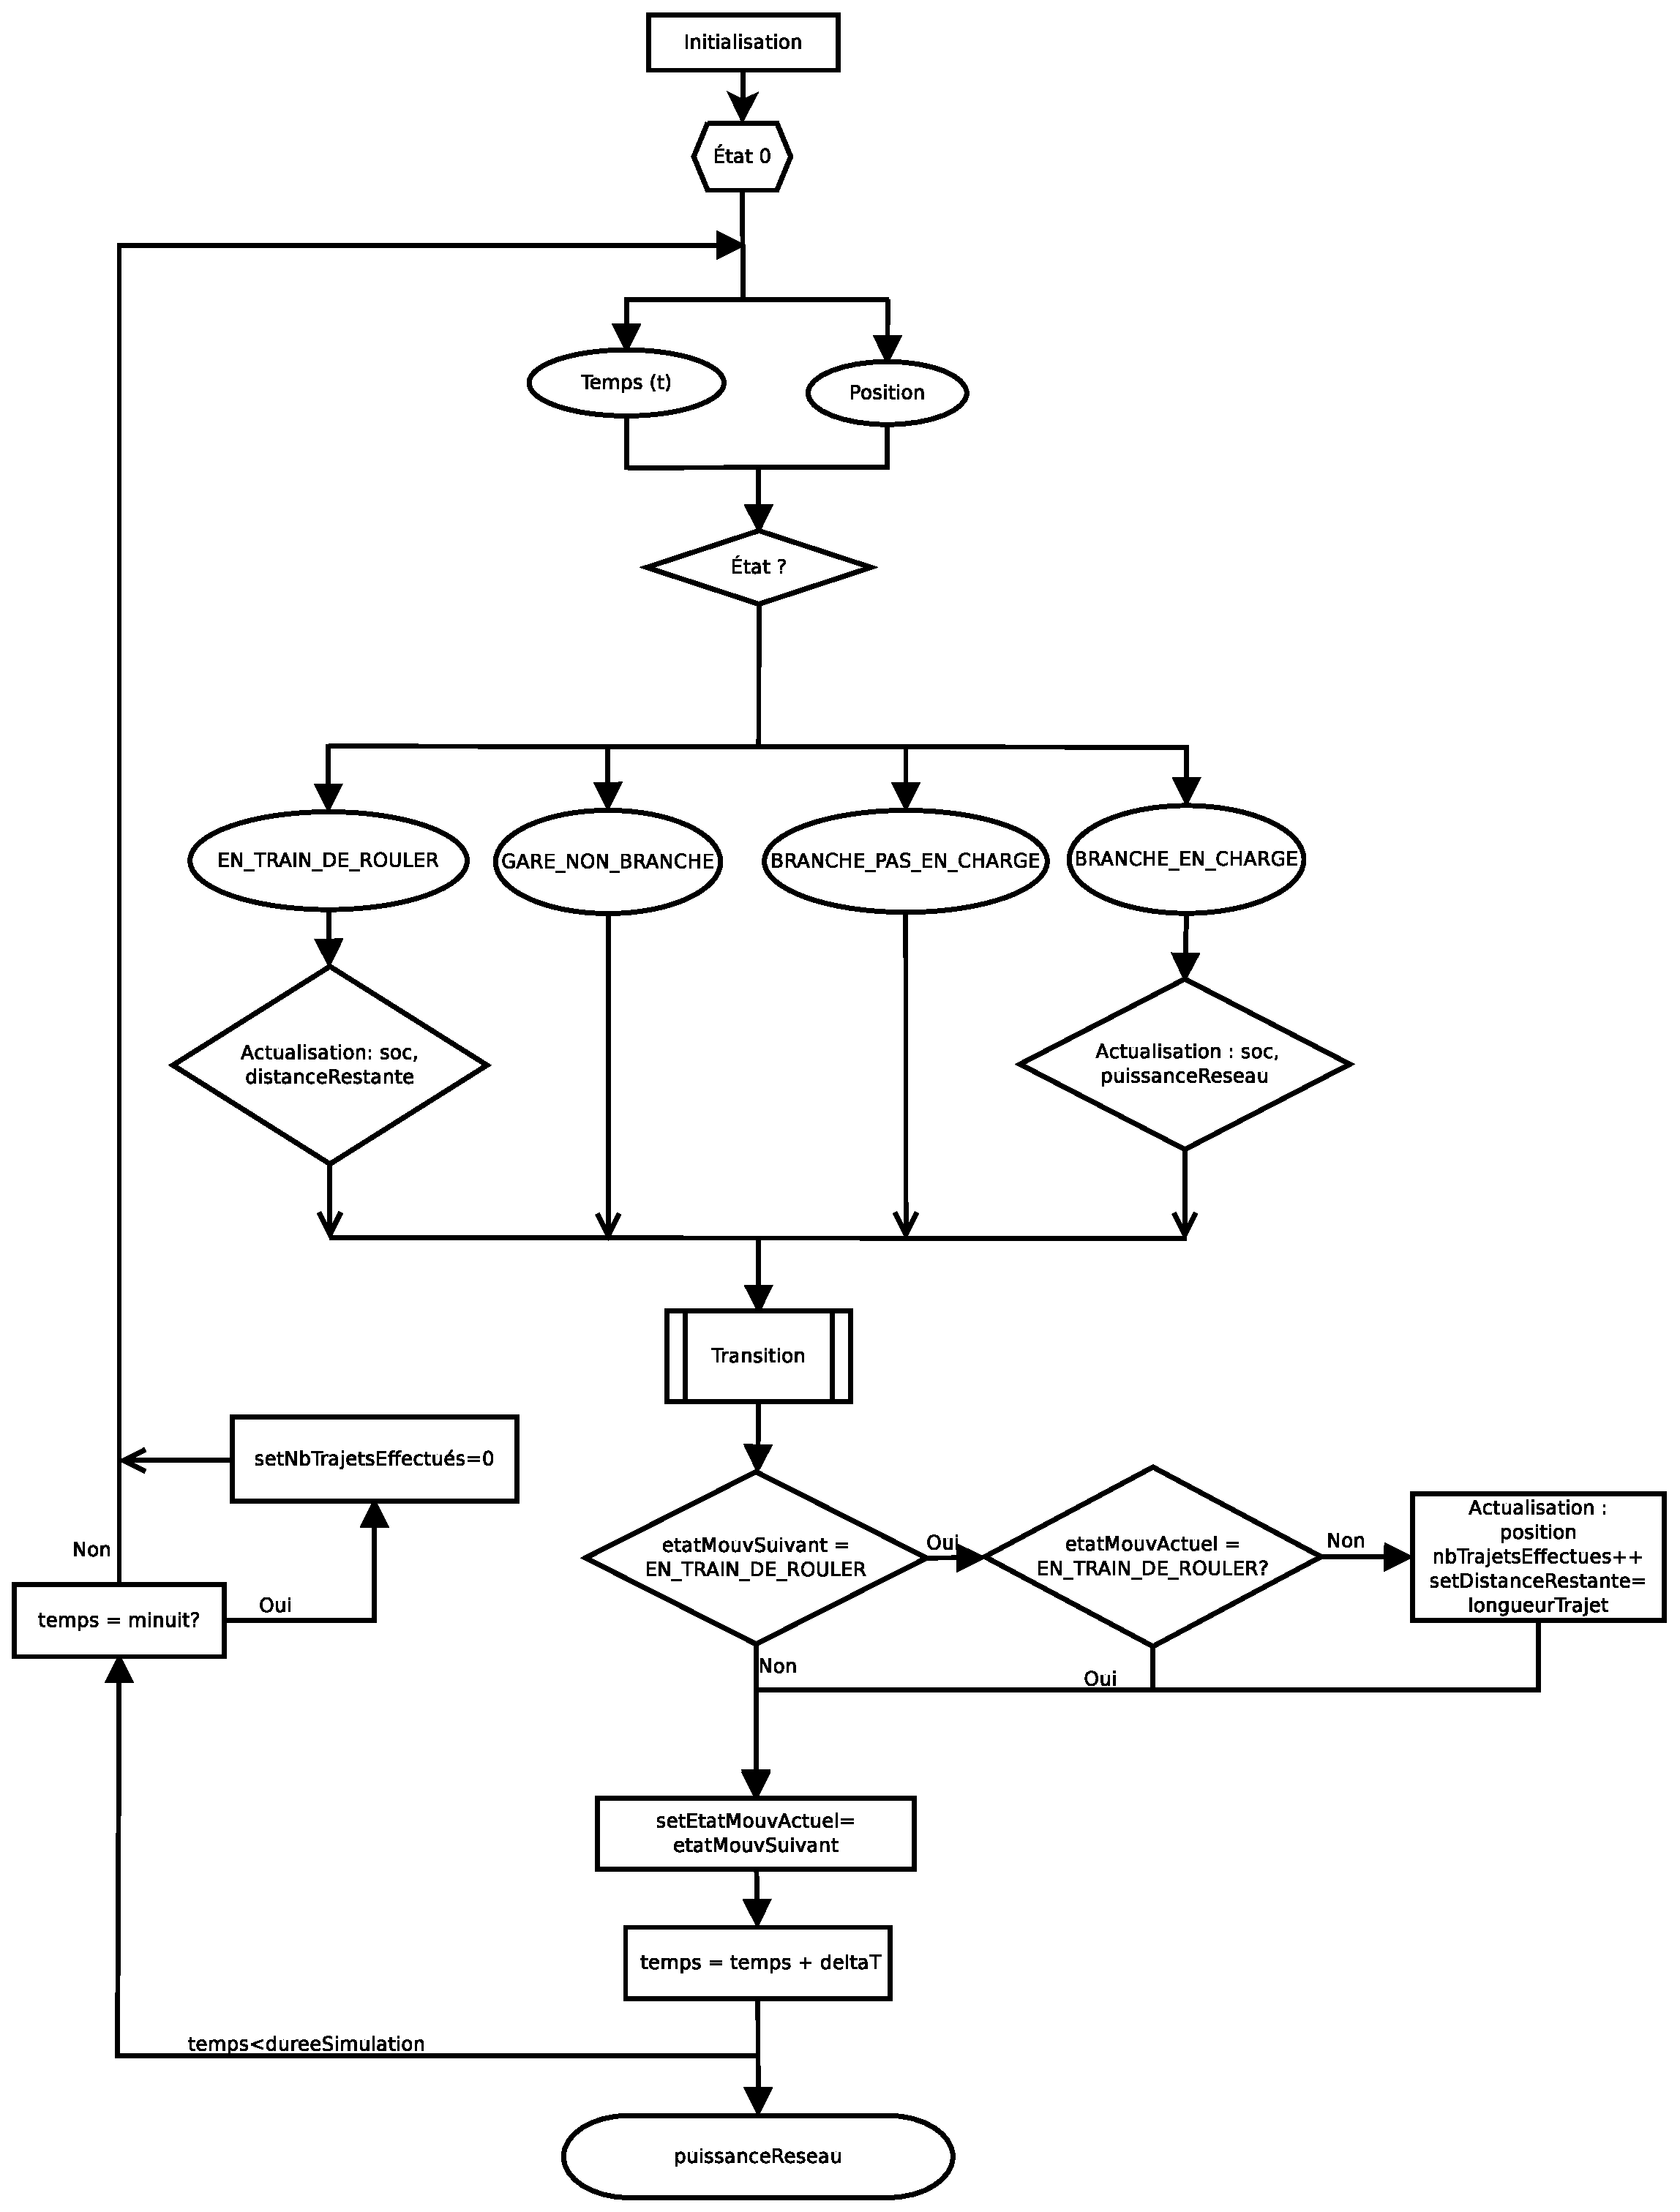
\includegraphics[height=0.9\textheight]{fig/flowPrincipal.eps}
				\caption{Logigramme de la méthode \lstinline{simulation}.\label{fig.flowPrincipal}}
			\end{figure}
			\begin{figure}
				\centering
				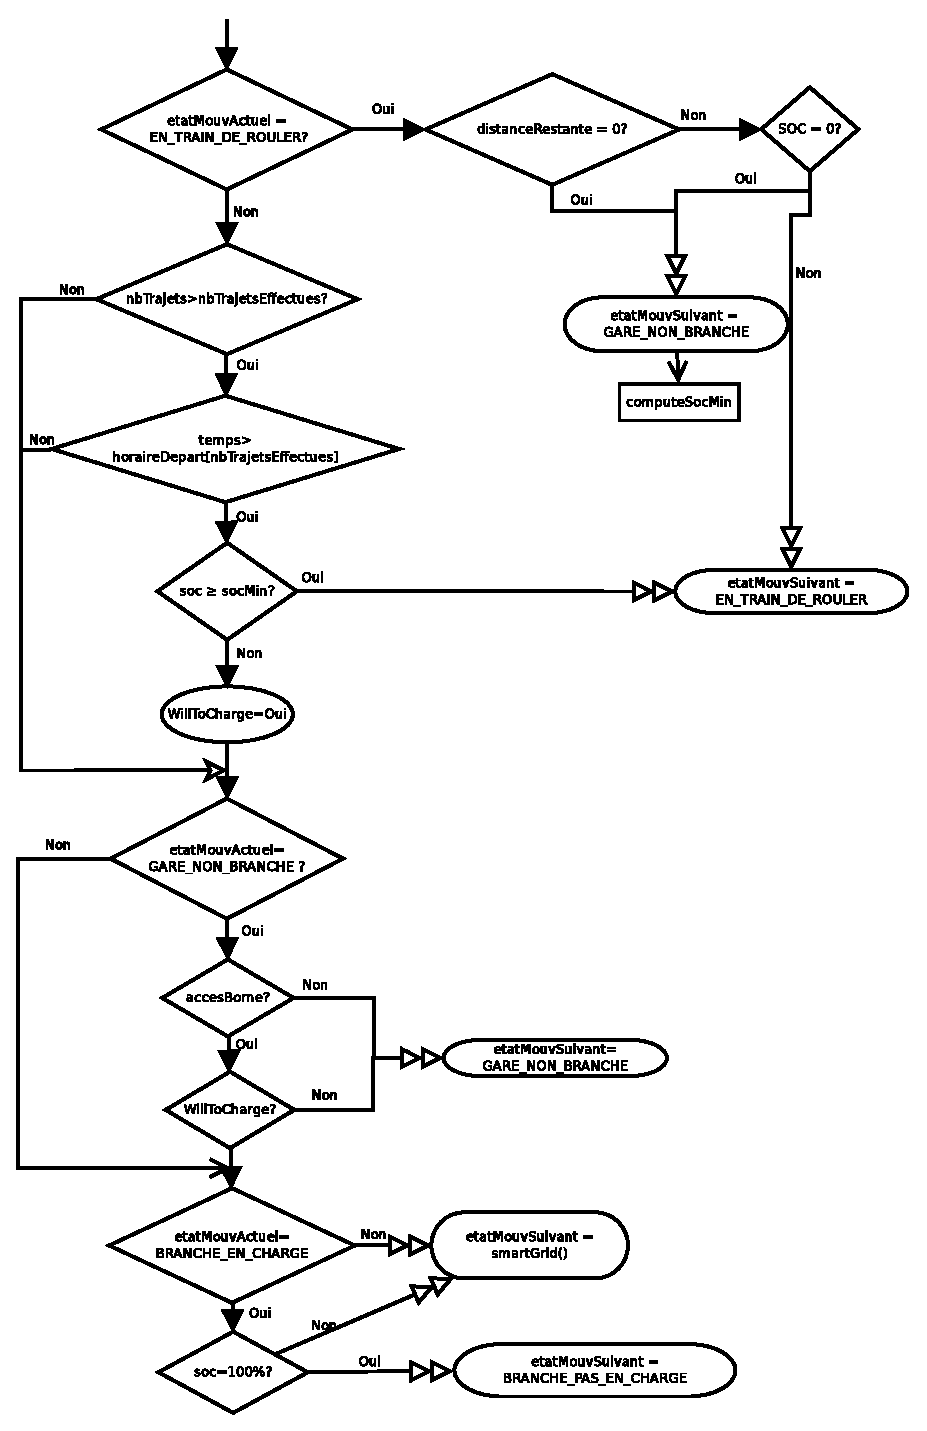
\includegraphics[height=0.9\textheight]{fig/flowTransition.eps}
				\caption{Bloc Transition.\label{fig.flowTransition}}
			\end{figure}
			
			Dans l’organigramme de la méthode \lstinline{transition} on observe deux variables qui n'ont pas encore été décrites.
			
			La première, \lstinline{willToCharge}, est un booléen qui décrit de manière sommaire le comportement de l'utilisateur. On fait l'hypothèse d'un utilisateur rationnel qui ne met son véhicule en charge que lorsque l'autonomie de celui-ci ne lui permet pas de faire les trajets à venir. On simule ainsi le comportement réel des utilisateurs qui, d'après nos données, ne chargent pas leur véhicule de manière systématique, mais en moyenne tous les trois jours.
			
			La deuxième est la fonction 
			\begin{lstlisting}		
    int Vehicule::smartGrid(int temps, int deltaT, int usecase)		
            \end{lstlisting}		
			Cette fonction est définie pour prendre en compte tous les aspects de \smartgrid{}, \emph{Vehicle to Grid}, effacement de charge, etc. C'est dans cette fonction que sont implémentés les différents cas possibles (\emph{use cases}) de monitoring de la charge d'un véhicule. Les \emph{use cases} que nous avons utilisés, et leur implémentation, sont décrits dans la paragraphe~\vref{sec.useCases}. 
			
			D'un point de vue technique, cette fonction retourne un entier qui correspond à un état de charge (\lstinline{BRANCHE_EN_CHARGE} ou \lstinline{BRANCHE_PAS_EN_CHARGE}) selon l'état du véhicule et la méthode d'effacement utilisée, et lève un marqueur qui indique à la suite de la fonction \lstinline|simulation| si le véhicule courant fait du \emph{Vehicle2Grid}. Cette méthode sera le plus souvent imposée par le fournisseur d’électricité dans la réalité.
			
			\bigskip
			
			Lors de l'appel de la fonction \lstinline{main}, la fonction principale du programme, celle-ci prend différents arguments :
			\begin{itemize}
			\item la longueur du pas de temps, $\delta t$ (variable \lstinline{deltaT}), en minutes;
			\item le nombre $D$ de jours correspondant à la durée de la simulation;
			\item le nombre $N$ de véhicules à générer pour la simulation;
			\item le nombre $I$ d'itérations de du programme (on effectue plusieurs fois la même simulation et on moyenne la puissance obtenue).
			\end{itemize}
			
			Le tableau \lstinline{puissanceReseau}, de taille $D \times 1440 / \delta t$ et indexé par les pas de temps de la simulation, est ensuite initialisé. Chaque case contiendra la puissance requise par l'ensemble de la flotte modélisée pour se recharger à l'instant correspondant.
			
			Ensuite la fonction est basiquement une double boucle :
			\begin{enumerate}
			\item une première boucle sur la taille de l'échantillon, qui génère un véhicule par étape et le fait passer dans la deuxième boucle ;
			\item la deuxième boucle est celle décrite dans l'organigramme \vref{fig.flowPrincipal}, indexée par les pas de temps successifs, où à chaque itération la fonction \lstinline{simulation} augmente la valeur la case correspondante de \lstinline{puissanceReseau} d'une unité de puissance ou pas selon que le véhicule est en charge ou non.
			\end{enumerate}
			
			En sortie, on obtient donc un tableau contenant toutes les informations nécessaires au tracé de la courbe de charge imposée par cette flotte au cours du temps.
			
			Après avoir discuté des différents cas de figure que nous avons étudié, c'est cette courbe que nous allons analyser.
			
			%
\begin{tikzpicture}
% style des noeuds
\tikzstyle{etat} = [ellipse, draw]
\tikzstyle{test} = [rectangle, draw]
\tikzstyle{instruct} = [rectangle, draw, rounded corners=4pt]
% style des flèches
\tikzstyle{suite} = [->, >=stealth', thick, rounded corners=4pt]

%% placement des noeuds
\node[instruct] (initialisation) at (0,0) {Initialisation};
\node[etat] (etat0) at (0,-1) {Etat $t$};
\node[test] (whichState) at (0,-2) {etatMouvement ?};
%
%% placement des flèches
\draw[suite] (initialisation) -- (etat0);
\draw[suite] (etat0) -- (whichState);
\end{tikzpicture}
		
		
		\clearpage
		\subsection{  Bornes de recharge et \emph{use case} } \label{sec.useCases}
		
		Nous avons plusieurs possibilités de prédiction en ce qui concerne les infrastructures de recharge. En effet celles-ci peuvent avoir différentes répartitions géographiques sur le territoire (seulement au domicile des utilisateurs ou bien aussi sur leur lieu de travail par exemple).
		De plus il y a aussi différentes possibilités d'implémentation du système \smartgrid{}. Par exemple il peut ne pas y avoir de \smartgrid{} du tout ou bien il peut y avoir un système de \emph{Vehicle to Grid}.
		Nous allons ainsi définir des \textit{use case} (cas d'utilisations) pour les bornes de recharge. 
		
		Nous avons retenu trois scénarios en ce qui concerne la répartition des bornes de recharge :
		\begin{enumerate}
			\item dans la quasi-totalité des cas (\SI{96}{\percent}), une borne au domicile, \SI{33}{\percent} des véhicules possèdent une borne au travail et \SI{14}{\percent} fréquentent des lieux publics où se trouve une borne; cette répartition correspond à la situation actuelle (données statistiques);
			\item les domiciles sont toujours équipés, les entreprises font des efforts et la voie publique s'équipent sur la moitié du territoire;
			\item le véhicule électrique s'est démocratisé : les domiciles sont équipés d'une borne, la majorité des entreprises en proposent à leurs employés et on en trouve sur \SI{90}{\percent} du territoire public.
		\end{enumerate}
		
		\bigskip
		
		On définit aussi différents cas d'utilisation des bornes de recharge en ce qui concerne le \smartgrid{}:
		\begin{enumerate}
			\item pas d'implémentation du \smartgrid{}, on recharge la voiture dès qu'elle est branchée, jusqu'à ce que la batterie soit à sa charge maximale;
			\item on ne recharge pas les voitures pendant les pics de consommation, c'est-à-dire entre 18 heures et 21 heures;
			\item on implémente le système \emph{Vehicle to Grid}, c'est-à-dire qu'entre 18 heures et 21 heures on ne recharge pas mais en plus les véhicules dont l'état de charge est supérieur à \lstinline{socMin} servent à alimenter le réseau en énergie. On considère que c'est l'utilisateur qui rentre ce \lstinline{socMin} dans la borne.  Après 21 heures la recharge normale des véhicules peut reprendre. Nous avons effectué l'hypothèse que ces véhicules en \emph{Vehicle to Grid} fournissent une puissance de \SI{2}{\kilo\watt}. En effet, la rétrocession de l'énergie de la batterie n'atteint pas, avec les technologies actuelles, \SI{100}{\percent}.
		\end{enumerate}
		Notons que tous les usagers de véhicules électriques n'acceptent pas forcément de participer au \smartgrid{} ou encore au \emph{Vehicle to Grid}. On a donc fait l'hypothèse que \SI{75}{\percent} des utilisateurs accepteraient de ne pas recharger leur véhicule durant le pic de consommation et que \SI{66}{\percent} de ces utilisateurs accepteraient de rétrocéder de l'énergie au réseau durant cette période.
		
		\bigskip
		
		Tous ces cas d'utilisations sont volontairement larges et sans nuances afin d'avoir une large fourchette de résultats.
		
		\subsection{Résultats}
			
			\begin{figure}[!h]
				\centering
				\begin{tikzpicture}
					\begin{axis}[
					/pgf/number format/.cd,
					use comma,
					1000 sep={ },
					height = 8cm,
					width = 15cm,
					axis x line = bottom,
					ymin = 0,
					axis y line = left,
				 	xlabel = Heures,
				 	ylabel = Consommation (MW)
				 	]
					\addplot[mark = , smooth, color=blue] table[x=Heures,y=2015-01-21] {fig/courbesRTE.txt};
					\addlegendentry{21/01/2015};
					\addplot[mark =, smooth, color=red] table[x=Heures,y=2014-07-17] {fig/courbesRTE.txt};
					\addlegendentry{17/07/2014}
					\end{axis}
				\end{tikzpicture}
				\caption{Courbe de charge du réseau français un jour d'hiver (en bleu) et un jour d'été (en rouge)}
			\end{figure}
			
			\subsubsection{Cas de référence}
			
			Dans l'ensemble de nos modélisations nous avons essayé de partir d'une modélisation de référence et d'en modifier que un ou deux paramètres pour pouvoir comparer aisément les différents résultats obtenus.
			
			Voici les paramètres de ce cas de référence :
			\begin{table}[h!]
			\centering
			\begin{tabular}{|c|c|}
			\hline
			Nombre de Véhicule ($N$) & 163000 \\
			\hline
			\lstinline|deltaT| & \SI{2}{\min} \\
			\hline
			Durée de la simulation & 5 jours \\
			\hline
			Nombre d'itérations & 4 \\
			\hline
			\end{tabular}
			\end{table}
			Le nombre d'itérations correspond au nombre de fois ou nous faisons tourner la boucle de simulation avec $N$ véhicules, et la courbe obtenue est la moyenne des résultats des différentes itérations.
			
			\subsubsection{Influence de l'état de charge initial}
				
				Nous avons tout d'abord étudié l'influence de l'état de charge initial pris en compte dans notre modèle. En effet, il était important de savoir si un choix arbitraire d'état de charge initial influencé grandement ou non nos résultats.
					
				Nous avons donc effectué une première série de modélisation avec les paramètres suivants :
				\begin{table}[h!]
				\centering
				
				\begin{tabular}{|c||c|}
					\hline
					& \lstinline|soc| initial\\
					\hline
					Cas 1 & 100\% \\
					\hline
					Cas 2 & 75\%\\
					\hline
					Cas 3 & 50\%\\
					\hline
					Cas 4 & 25\%\\
					\hline
					Cas 5 & 0\%\\
					\hline
				\end{tabular}
				\end{table}
				Dans ces modélisations, il n'y a aucun \emph{use case} d'utilisé, la fonction \lstinline|smartGrid| retourne la valeur \lstinline|BRANCHE_EN_CHARGE| si la voiture n'est pas pleinement chargé, \lstinline|BRANCHE_PAS_EN_CHARGE| si non.
				
				Les courbes présentées sur la figure \vref{fig.socInitVariable} sont celles obtenues au cinquième jour de modélisation.
				
				\begin{figure}[!h]
					\centering
					\begin{tikzpicture}
						\begin{axis}[
						/pgf/number format/.cd,
						use comma,
						1000 sep={ },
						height = 8cm,
						width = 15cm,
						axis x line = bottom,
						axis y line = left,
						xlabel = Heures,
						ylabel = Consommation (kW)
						]
						\addplot[mark = , smooth, color=blue] file{fig/socInitVariables/cas1-100.csv};
						\addlegendentry{Cas 1};
						\addplot[mark = , smooth, color=violet] file{fig/socInitVariables/cas2-075.csv};
						\addlegendentry{Cas 2};
						\addplot[mark = , smooth, color=yellow] file{fig/socInitVariables/cas3-050.csv};
					\addlegendentry{Cas 3};
						\addplot[mark = , smooth, color=cyan] file{fig/socInitVariables/cas4-025.csv};
					\addlegendentry{Cas 4};
						\addplot[mark = , smooth, color=red] file{fig/socInitVariables/cas5-000.csv};
					\addlegendentry{Cas 5};
						\end{axis}
					\end{tikzpicture}
					\caption{Effet de l'état de charge initial sur la courbe de charge résultat au bout de 5 jours. \label{fig.socInitVariable}}
				\end{figure}			
				
				On constate que quelque soit l'état initial choisi il y a convergence des modélisation au bout d'un temps suffisamment long. Cela nous permet de choisir arbitrairement un état de charge initial de \SI{100}{\percent} pour le reste de nos modélisations sans que cette décision n'impacte sur la généralité de notre étude. 
		
				
				\subsubsection{Influence de la répartition des bornes}
				
				Nous avons aussi étudié l'influence de la répartition des bornes sur l'allure de la courbe de charge.
				
				Une fois encore nous avons comparés au cinquième jour de modélisation différents cas : 
				\begin{table}[h!]
				\centering
				\begin{tabular}{|c||c|c|c|}
					\hline
					Nombre de bornes pour 100 véhicules & À la maison & Lieu de travail & Lieu public \\
					\hline
					Cas 1 & 96 & 33 & 14 \\
					\hline
					Cas 2 & 98 & 66 & 50\\
					\hline
					Cas 3 & 99 & 80 & 95\\
					\hline
				\end{tabular}
				\end{table}		
				
				Le cas 1 correspond à la situation actuelle pour les détenteurs de véhicules électriques.
				
				Les courbes sont présentés en figure \vref{fig.repartitionBornes}. Comme dans le cas précédent, aucune implémentation de \smartgrid{} n'est mise en place.
				
				\begin{figure}[!h]
					\centering
					\begin{tikzpicture}
						\begin{axis}[
						/pgf/number format/.cd,
						use comma,
						1000 sep={ },
						height = 8cm,
						width = 15cm,
						axis x line = bottom,
						axis y line = left,
						xlabel = Heures,
						ylabel = Consommation (kW)
						]
						\addplot[mark = , smooth, color=blue] file{fig/repartitionBornes/cas1-963314.csv};
						\addlegendentry{Cas 1};
						\addplot[mark = , smooth, color=violet] file{fig/repartitionBornes/cas2-986650.csv};
						\addlegendentry{Cas 2};
						\addplot[mark = , smooth, color=yellow] file{fig/repartitionBornes/cas3-998095.csv};
						\addlegendentry{Cas 3};
						\end{axis}
					\end{tikzpicture}
					\caption{Effet de la répartition des bornes sur la courbe de charge. \label{fig.repartitionBornes}}
				\end{figure}
				
				
				
				\subsubsection{Influence de la mise en place des systèmes \smartgrid{} et \emph{Vehicle to Grid}}
				
				Ici, nous étudions le profil de la courbe de charge lorsque nous implémentons le \smartgrid{} et le \emph{Vehicle to Grid}.
				
				Le cas 1 correspond à notre étude de référence, dans laquelle une flotte de 163000 véhicules est observée sur une durée de 5 jours.
				
				Le cas 2 est la mise en place du \smartgrid{}: on considère que \SI{75}{\percent} des véhicules électriques sont concernés par ce procédé, c'est-à-dire qu'ils acceptent de ne pas se recharger entre \SI{18}{\hour} et $\SI{18}{\hour}+H$ où $H$ est une variable aléatoire uniforme dont la valeur est comprise entre 0 et 3.
				
				Le cas 3 est la mise place du \emph{Vehicle to Grid}: on considère que \SI{66}{\percent} des véhicules électriques qui ont accepté le \smartgrid{} (cas précédent) sont concernés par ce procédé, c'est-à-dire que non seulement ils ne se rechargent pas, mais en plus fournissent une puissance de \SI{2}{\kilo\watt} au réseau électrique, durant la même période que dans le cas précédent.
				
				Les résultats sont présentés sur la figure \vref{fig.usecases}.
				
				\begin{figure}[!h]
					\centering
					\begin{tikzpicture}
						\begin{axis}[
						/pgf/number format/.cd,
						use comma,
						1000 sep={ },
						height = 8cm,
						width = 15cm,
						axis x line = bottom,
						axis y line = left,
						xlabel = Heures,
						ylabel = Consommation (kW)
						]
						\addplot[mark = , smooth, color=blue] file{fig/useCases/cas1.csv};
						\addlegendentry{Cas 1};
						\addplot[mark = , smooth, color=violet] file{fig/useCases/cas2.csv};
						\addlegendentry{Cas 2};
						\addplot[mark = , smooth, color=yellow] file{fig/useCases/cas3.csv};
						\addlegendentry{Cas 3};
						\end{axis}
					\end{tikzpicture}
					\caption{Effet de la mise en place des systèmes \smartgrid{} et \emph{Vehicle to Grid} sur la courbe de charge. \label{fig.usecases}}
				\end{figure}
				
				

				
				
			
		\subsection{Difficultés rencontrées}
		
		
